\chapter{Analiza danych genomicznych}\label{chap5}
\begin{flushright}
\textit{Tke key is to understand genomics \\
to improve cancer care. \\
The Cancer Genome Atlas Study
}
\end{flushright}

Niniejszy rozdział poświęcony jest analizie danych genomicznych. W podrozdziale \ref{cha:gen} przedstawiono pokrótce genetyczne podstawy nowotworzenia, które szerzej opisane są w cytowanej literaturze. W podrozdziale \ref{chan:TCGA} opisano schemat \textit{The Cancer Genome Atlas} (TCGA), badania z którego zaczerpnięto dane do analizy biostatystycznej. Analiza przeżycia polegająca na zastosowaniu modelu Coxa, dla którego estymacja współczynników odbywa się metodą stochastycznego spadku gradientu (opisaną w rozdziale \ref{rozdz4}) zaprezentowana została wraz z komentarzami w podrozdziale \ref{chap:analiza}. 

W ramach analizy starano się ocenić wpływ mutacji poszczególnych genów na przeżywalność pacjentów. Celem analizy było uzyskanie odpowiedzi na pytanie czy istnieją geny, które zmutowane powodują, że ryzyko wystąpienia zdarzenia jakim jest zgon w wyniku choroby nowotworowej jest większe w grupach pacjentów bez mutacji w danym genie. Aby zweryfikować hipotezę na tak obszernych danych zdecydowano się zastosować metodę strumieniowej estymacj współczynników w modelu Coxa przy pomocy stochastycznego spadku gradientu, której stworzenie było głównym założeniem pracy, gdyż tradycyjna metoda zaimplementowana w funkcji \texttt{coxph} w pakiecie \texttt{survival} \cite{survival} nie jest przystosowana do tak dużych zbiorów danych jak te z TCGA. Z racji na zbyt dużą ilość genów (przekraczającą kilkanaście tysięcy), które mogłyby być zmutowane i wzięte do analizy jako zmienna objaśniająca czas do zdarzenia, niemożliwe byłoby wyestymowanie współczynników modelu standardową metodą.

Wielką zaletą modelu Coxa z estymacją przy użyciu metody stochastycznego spadku gradientu jest możliwość zastosowania go do zbiorów danych o rozmiarze zmiennych znacznie przekraczającym wymiar obserwacji. Zaprezentowana w rozdziale \ref{implemento} implementacja pozwala w skończonym czasie znaleźć współczynniki modelu odpowiadające za wpływ danych genów na śmiertelność pacjentów w chorobach nowotworowych. Jest to nie tylko zdobycz obliczeniowa ale także ważne narzędzie w analizach biostatystycznych danych dużej skali, które z powodzeniem może zostać wykorzystywane do analizy ludzkiego genomu, tak by w przyszłości poszerzać zrozumienie procesów mutacji zachodzących w ludzkim organizmie, dzięki którym możliwe byłoby skuteczniejsze leczenie chorób nowotworowych.
\newpage
\section{Genetyczne podstawy nowotworzenia}\label{cha:gen}
Choroby nowotworowe stanowią drugą, po chorobach serca, przyczynę zachorowań i zgonów na całym świecie. Wyniki opracowane przez Polską Unię Onkologiczną wskazują na tendencję wzrostową liczby zachorowań na nowotwory i rokują na utrzymanie się jej do 2020~\cite{zikula}.

Według współczesnej definicji \textbf{nowotwór} jest \textit{chorobą cyklu komórkowego} i oznacza \cite{zikula2} \\ \ \\ \textit{nieprawidłową tkankę, która powstała z jednej komórki i rośnie jako następstwo zaburzeń dynamizmu i prawidłowego przebiegu cyklu komórkowego oraz zaburzeń różnicowania się komórki i komunikacji wewnątrzkomórkowej, międzykomórkowej i pozakomórkowej jej klonalnego potomstwa}. \\ \ \\
Wyniki badań nad transformacją nowotworową wykazały, że nowotwory powstają jako wynik wielu mutacji w DNA komórki somatycznej, które poprzez akumulację wywołują utratę kontroli nad proliferacją (rozwojem), wzrostem i różnicowaniem~\cite{zikula5}.

Proces tworzenia nowotworu (\textbf{kancerogeneza}) jest wieloczynnikowy i wielostopniowy, a~zmiany w nim nasilają się w miarę pogłębiania się niestabilności genetycznej \cite{zikula2}. Transformacja nowotworowa następuje w wyniku zmian powstałych w obrębie czterech różnych kategorii genów, które wpływają na proliferację i różnicowanie komórek \cite{zikula}. Czynniki genetyczne zaangażowane w systemy naprawy DNA, a także w procesy proliferacji i różnicowania komórek \cite{zikula4} można podzielić na:  
\begin{itemize}
\item \textit{geny regulujące naprawę uszkodzonego DNA} - mechanizmy szybkiej naprawy DNA zapobiegają przed mutacjami genów odpowiedzialnyh m. in. za proliferację i różnicowanie się komórek. Geny biorące udział w naprawie DNA nie są onkogenne, natomiast mutacje w ich obrębie mogą ułatwić transformację nowotworową oraz podwyższają ryzyko utrwalenia się zmian w pozostałych grupach i dlatego mają podstawowe znaczenie dla integracji genomu.
\item \textit{geny supresorowe} (antyonkogeny) - kontrolują cykl komórkowy. Są punktami kontrolnymi pomiędzy fazami cyklu komórkowego, zapobiegają niekontrolowanym podziałom komórkowym oraz są czynnikami negatywnej kontroli podziałów.
\item \textit{protoonkogeny} - potencjalnie zdolne do wyzwolenia procesu transformacji nowotworowej. Uwarunkowana mutacją zmiana ich ekspresji sprawia, że przekształcają się w~onkogeny, czyli geny bezpośrednio aktywujące transformację nowotworową.
\item \textit{geny regulujące apoptozę} (naturalny proces zaprogramowanej śmierci komórki w organizmach wielokomórkowych) - zahamowanie procesu apoptozy wskutek mutacji czynników indukujących wydłuża okres życia komórek, zwiększając tym samym populację komórek narażonych na działanie karcynogenów i prawdopodobieństwo wystąpienia mutacji w komórce.
\end{itemize}
Zmiany genetyczne w komórkach zachodzą pod wpływem działania czynników mutagennych, do których można zaliczyć: promieniowanie UV (czynniki fizyczne), substancje obecne w dymie papierosowym i spalinach samochodowych, azbest, promieniowanie jonizujące, temperatura i niektóre metale ciężkie (czynniki chemiczne), wirusy, toksyny bakteryjne i pasożytnicze czy pośrednie produkty przemiany materii (czynniki biologiczne)~\cite{zikula3}.


\section{Projekt The Cancer Genome Atlas}\label{chan:TCGA}

Do analizy wykorzystano dane udostępniane w ramach \textit{The Cancer Genome Atlas}~\cite{broad}. The~Cancer~Genome Atlas (TCGA) to kompleksowy projekt o skoordynowanych wysiłkach, mający na celu przyśpieszenie zrozumienia molekularnych podstaw nowotworu. Ma się to odbywać poprzez stosowanie technologii analizy danych dużej skali do udostępnianych danych genomicznych i zsekwencjonowanego genomu tkanek nowotworowych. TCGA to inicjatywa \textit{National Cancer Institute} (NCI) oraz \textit{National Human Genome Research Institute} (NHGRI), czyli 2 z pośród 27 instytutów i centrów Narodowego Instytutu Zdrowia w Departamencie Zdrowia i Opieki Społecznej Stanów Zjednoczonych.

Jak podaje \cite{patrycja}, w biologii jest znane ponad 200 różnych form nowotworu i jeszcze więcej ich podtypów. Każdy z nich wywołany jest nieprawidłowościami w DNA, które sprawiają, że komórki namnażają się w sposób niekontrolowany. Identyfikując zmiany w kompletnym zbiorze DNA (genomie) dla każdego nowotworu i wiedząc jak te zmiany wpływają na jego rozwój, możliwe będzie skuteczne zapobieganie nowotworom, wczesne ich wykrywanie~i~leczenie. 

Nadrzędnym celem TCGA jest poprawienie naszej zdolności do diagnozowania, leczenia i profilaktyki nowotworów. TCGA aby osiągnąć ten cel w sposób naukowo rygorystyczny, początkowo jako projekt pilotażowy, opracowało i przetestowało strukturę badawczą konieczną do systematycznego badania całego spektrum zmian genomu zawartych w ponad 20 rodzajach raka.

Dzięki projektowi TCGA społeczność naukowców walczących z rakiem może korzystać z~danych uzyskanych z sekwencjonowania komórek pochodzących z tkanek nowotworowych zebranych przez \textit{Cancer Genomics Hub} (CGHub) i \textit{Genome Data Analysis Centers}~(GDACs). Te i~wiele więcej instytucji opisanych szerzej jest w \cite{patrycja}. TCGA Genome Data Analysis Centers składają się z 7 instytucji, a jedna z nich \textit{Broad Institute, Cambridge} udostępnia dane oraz wyniki swoich analiz poprzez portal Firehose Broad GDAC (\texttt{http://gdac.broadinstitute.org/}). Portal udostępnia dane dla 38 kohort związanych z występującym typem nowotworu. Więcej na temat kohort i danych zawartych w TCGA można znaleźć w~\cite{chin1}, \cite{chin2}, \cite{future} czy \cite{patrycja}. 

Dane z TCGA pobrano przy użyciu pakietu \texttt{RTCGA} \cite{kosa1} i umieszczono w pakietach
\begin{itemize}
\item \texttt{RTCGA.clinical} \cite{kosa2}, zawierającym dane kliniczne o pacjentach,
\item \texttt{RTCGA.mutations} \cite{kosa3}, zawierającym dane o występujących w genach mutacjach
\end{itemize} 
oraz zostały one wykorzystane w następnym rozdziale do sprawdzenia czy występowanie mutacji w danym genie ma wpływ na przeżywalność pacjentów dotkniętych nowotworem.

\newpage

\section{Analiza wpływu mutacji genów na czas życia}\label{chap:analiza}

Do analizy badającej wpływ występowania mutacji genów na czas przeżycia
wykorzystano dane kliniczne i dane o występujących u pacjentów mutacjach
genetycznych. Starano się wykorzystać dane ze wszystkich 38 dostępnych
kohort nowotworowych z badania \textit{The Cancer Genome Atlas} (TCGA),
jednak nie dla wszystkich kohort umieszczono w badaniu dane o mutacjach.
Częśc wspólną nazw dla kohort zawierających zarówno dane kliniczne oraz
dane o mutacjach wygenerowaną dzięki wywołaniu

\begin{Shaded}
\begin{Highlighting}[]
\NormalTok{(}\KeywordTok{extractCohortIntersection}\NormalTok{() ->}\StringTok{ }\NormalTok{cohorts)}
\end{Highlighting}
\end{Shaded}

\begin{verbatim}
 [1] "ACC"      "BLCA"     "BRCA"     "CESC"     "CHOL"     "COAD"    
 [7] "COADREAD" "DLBC"     "ESCA"     "GBM"      "GBMLGG"   "HNSC"    
[13] "KICH"     "KIPAN"    "KIRC"     "KIRP"     "LAML"     "LGG"     
[19] "LIHC"     "LUAD"     "LUSC"     "OV"       "PAAD"     "PCPG"    
[25] "PRAD"     "READ"     "SARC"     "SKCM"     "STAD"     "STES"    
[31] "TGCT"     "THCA"     "UCEC"     "UCS"      "UVM"     
\end{verbatim}

Następnie dla tak otrzymanych 35 kohort nowotworowych uzyskano dane o
statusie pacjenta (śmierć bądź cenzurowanie) oraz jego czasie spędzonym
pod obseracją dzięki funkcji

\begin{Shaded}
\begin{Highlighting}[]
\KeywordTok{head}\NormalTok{(}\KeywordTok{extractSurvival}\NormalTok{(cohorts) ->}\StringTok{ }\NormalTok{survivalData)}
\end{Highlighting}
\end{Shaded}

\begin{verbatim}
      bcr_patient_barcode patient.vital_status times
ACC.1        TCGA-OR-A5J1                    1  1355
ACC.2        TCGA-OR-A5J2                    1  1677
ACC.3        TCGA-OR-A5J3                    0  1942
ACC.4        TCGA-OR-A5J4                    1   423
ACC.5        TCGA-OR-A5J5                    1   365
ACC.6        TCGA-OR-A5J6                    0  2428
\end{verbatim}

Dane o mutacjach występujących wśród tkanek nowotworowych kolejnych
pacjentów uzyskano za pomocą

\begin{Shaded}
\begin{Highlighting}[]
\KeywordTok{extractMutations}\NormalTok{(cohorts, }\FloatTok{0.02}\NormalTok{) ->}\StringTok{ }\NormalTok{mutationsData}
\NormalTok{mutationsData[}\DecValTok{1}\NormalTok{:}\DecValTok{6}\NormalTok{, }\KeywordTok{c}\NormalTok{(}\DecValTok{1}\NormalTok{,}\DecValTok{4}\NormalTok{,}\DecValTok{56}\NormalTok{,}\DecValTok{100}\NormalTok{,}\DecValTok{207}\NormalTok{,}\DecValTok{801}\NormalTok{)]}
\end{Highlighting}
\end{Shaded}

\begin{verbatim}
  bcr_patient_barcode A2ML1 ALMS1 ATP2B2 CNTNAP4 PLEC
1     TCGA-02-0003-01     0     1      0       0    0
2     TCGA-02-0033-01     0     0      0       0    0
3     TCGA-02-0047-01     0     0      0       0    0
4     TCGA-02-0055-01     0     0      0       0    0
5     TCGA-02-2470-01     0     0      0       0    0
6     TCGA-02-2483-01     0     0      1       0    0
\end{verbatim}

gdzie wybrano jedynie te geny, których mutacja dotyczyła co najmniej 2
\% pacjentów mających zarówno dane kliniczne jak i dane o występujących
mutacjach w genach.

Dla tak otrzymanych dwóch zbiorów danych połączono dla pacjentów
informacje kliniczne z informacjami o mutacjach dzięki przypisanym do
pacjentów i ich próbek kodów \texttt{bcr\_patient\_barcode}, by
ostatecznie podzielić zbiór pacjentów na 100 losowo utworzonych grup.

\begin{Shaded}
\begin{Highlighting}[]
\KeywordTok{set.seed}\NormalTok{(}\DecValTok{4561}\NormalTok{)}
\KeywordTok{prepareCoxDataSplit}\NormalTok{(mutationsData,survivalData, }\DataTypeTok{groups =} \DecValTok{100}\NormalTok{) ->}\StringTok{ }\NormalTok{coxData_split}
\KeywordTok{head}\NormalTok{(coxData_split[[}\DecValTok{1}\NormalTok{]][}\KeywordTok{c}\NormalTok{(}\DecValTok{1}\NormalTok{,}\DecValTok{10}\NormalTok{), }\KeywordTok{c}\NormalTok{(}\DecValTok{210}\NormalTok{,}\DecValTok{302}\NormalTok{,}\DecValTok{356}\NormalTok{,}\DecValTok{898}\NormalTok{,}\DecValTok{911}\NormalTok{,}\DecValTok{1092}\NormalTok{:}\DecValTok{1093}\NormalTok{)])}
\end{Highlighting}
\end{Shaded}

\begin{verbatim}
     COL14A1 DOCK9 FASN SEMA5A SHPRH patient.vital_status times
81         0     0    0      0     0                    1     7
1068       1     0    0      1     0                    1  1171
\end{verbatim}

Niezbędną formułę modelu potrzebną do sprezycowania, które geny (a
pozostało ich 1091) należy uwzględnić w modelu uzyskano dzięki
pomocniczej funkcji

\begin{Shaded}
\begin{Highlighting}[]
\KeywordTok{prepareForumlaSGD}\NormalTok{(coxData_split) ->}\StringTok{ }\NormalTok{formulaSGD}
\end{Highlighting}
\end{Shaded}

Ostatecznie dla 6085 pacjentów, którzy posiadali informacje o
występujących mutacjach, oraz dla których odnotowano komplet i
poprawność danych klinicznych dotyczących statusu i obserwowanego czasu
przeżycia wyliczono wspólczynniki modelu proporcjonalnych hazardów Coxa
z wykorzystaniem stochastycznego spadku gradientu do estymacji. Model
dopasowano wielokrotnie z różnymi ciągami odpowiadającymi za długość
kroku algorytmu, dodatkowo badano różną ilość epok w algorytmie. Dla tak
powstałych kilku modeli wybrano ten, który dla swoich współczynników
dawał największą wartość funkcji częściowej log-wiarogodności dla
niewykorzystanej do uczenia próbki, zawierającej 2 ostatnie
zaobserwowane podzbiory obserwacji. Dla każdego z ciągów
\(1/t, 1/50\sqrt{t}, 1/100\sqrt{100}\) odpowiadających długościom
kroków w algorytmie wyznaczono współczynniki modelu dla 5 epok, dzięki
czemu możliwe było rozważanie postępu danego wariantu algorytmu również
po 1, 2, 3 czy 4 epokach.

\begin{Shaded}
\begin{Highlighting}[]
\NormalTok{coxData_split[}\DecValTok{99}\NormalTok{:}\DecValTok{100}\NormalTok{] ->}\StringTok{ }\NormalTok{testCox}
\NormalTok{coxData_split[}\DecValTok{1}\NormalTok{:}\DecValTok{98}\NormalTok{] ->}\StringTok{ }\NormalTok{trainCox}
\KeywordTok{coxphSGD}\NormalTok{(formulaSGD, }\DataTypeTok{data =} \NormalTok{trainCox, }\DataTypeTok{max.iter =} \DecValTok{490}\NormalTok{) ->}\StringTok{ }\NormalTok{model_1_over_t}
\KeywordTok{coxphSGD}\NormalTok{(formulaSGD, }\DataTypeTok{data =} \NormalTok{trainCox, }\DataTypeTok{max.iter =} \DecValTok{490}\NormalTok{,}
         \DataTypeTok{learningRates =} \NormalTok{function(t)\{}\DecValTok{1}\NormalTok{/(}\DecValTok{50}\NormalTok{*}\KeywordTok{sqrt}\NormalTok{(t))\}) ->}\StringTok{ }\NormalTok{model_1_over_50sqrt_t}
\KeywordTok{coxphSGD}\NormalTok{(formulaSGD, }\DataTypeTok{data =} \NormalTok{trainCox, }\DataTypeTok{max.iter =} \DecValTok{490}\NormalTok{,}
         \DataTypeTok{learningRates =} \NormalTok{function(t)\{}\DecValTok{1}\NormalTok{/(}\DecValTok{100}\NormalTok{*}\KeywordTok{sqrt}\NormalTok{(t))\}) ->}\StringTok{ }\NormalTok{model_1_over_100sqrt_t}
\end{Highlighting}
\end{Shaded}


Po dopasowaniu modeli sporządzono wykresy przedstawiające histogramy wartości współczynników modelu po każdej epoce, w rozróżnieniu na trzy typy ciągów odpowiedzialnych za długość kroku. Histogramy przedstawiono na Rysunkach \ref{fig:hist1} - \ref{fig:hist3}, zaś na Rysunku \ref{fig:hist4} przedstawiono ich porównanie na wspólnych osiach. Największe zróżnicowanie wśród współczynników modelu można zaobserwować dla modelu \texttt{model\_1\_over\_t}, w którym ciąg odpowiadający za długość kroku algorytmu to $1/t$. W pozostałych modelach współczynniki grupują się bliżej $0$ i rzadko co do modułu są większe od $0.5$. W przypadku modelu \texttt{model\_1\_over\_t} wartości współczynników bywają co do modułu niekiedy większa od 1. Oznaczać to może, że przy takim ciągu długości kroków, algorytm jest w stanie uwypuklić wpływ genów mających istotny wpływ na czas przeżycia pacjentów poprzez wyestymowanie większych wartości wśród odpowiednich współczynników. Różnice wśród wartości współczynników pomiędzy modelami najwyraźniej widać na Rysunku \ref{fig:hist4}, gdzie w przypadku modelu \texttt{model\_1\_over\_100sqrt\_t} ($\alpha_{model3} = 1/100\sqrt{t}$) pik w okolicach zera wskazuje na to, że mało genów można uznać za istotnie mające wpływ na czas przeżycia z powodu odpowiadających im współczynnikom bliskim $0$. Nie oznacza to jednak, że w tym przypadku model jest gorszy.

Zdecydowano się uznać za najlepszy ten model, który da największą wartość częściowej funkcji log-wiarogodności na testowym zbiorze wyznaczonym przez dwa ostatnie zaobserwowane podzbiory.  

\begin{figure}[!ht]
\centering
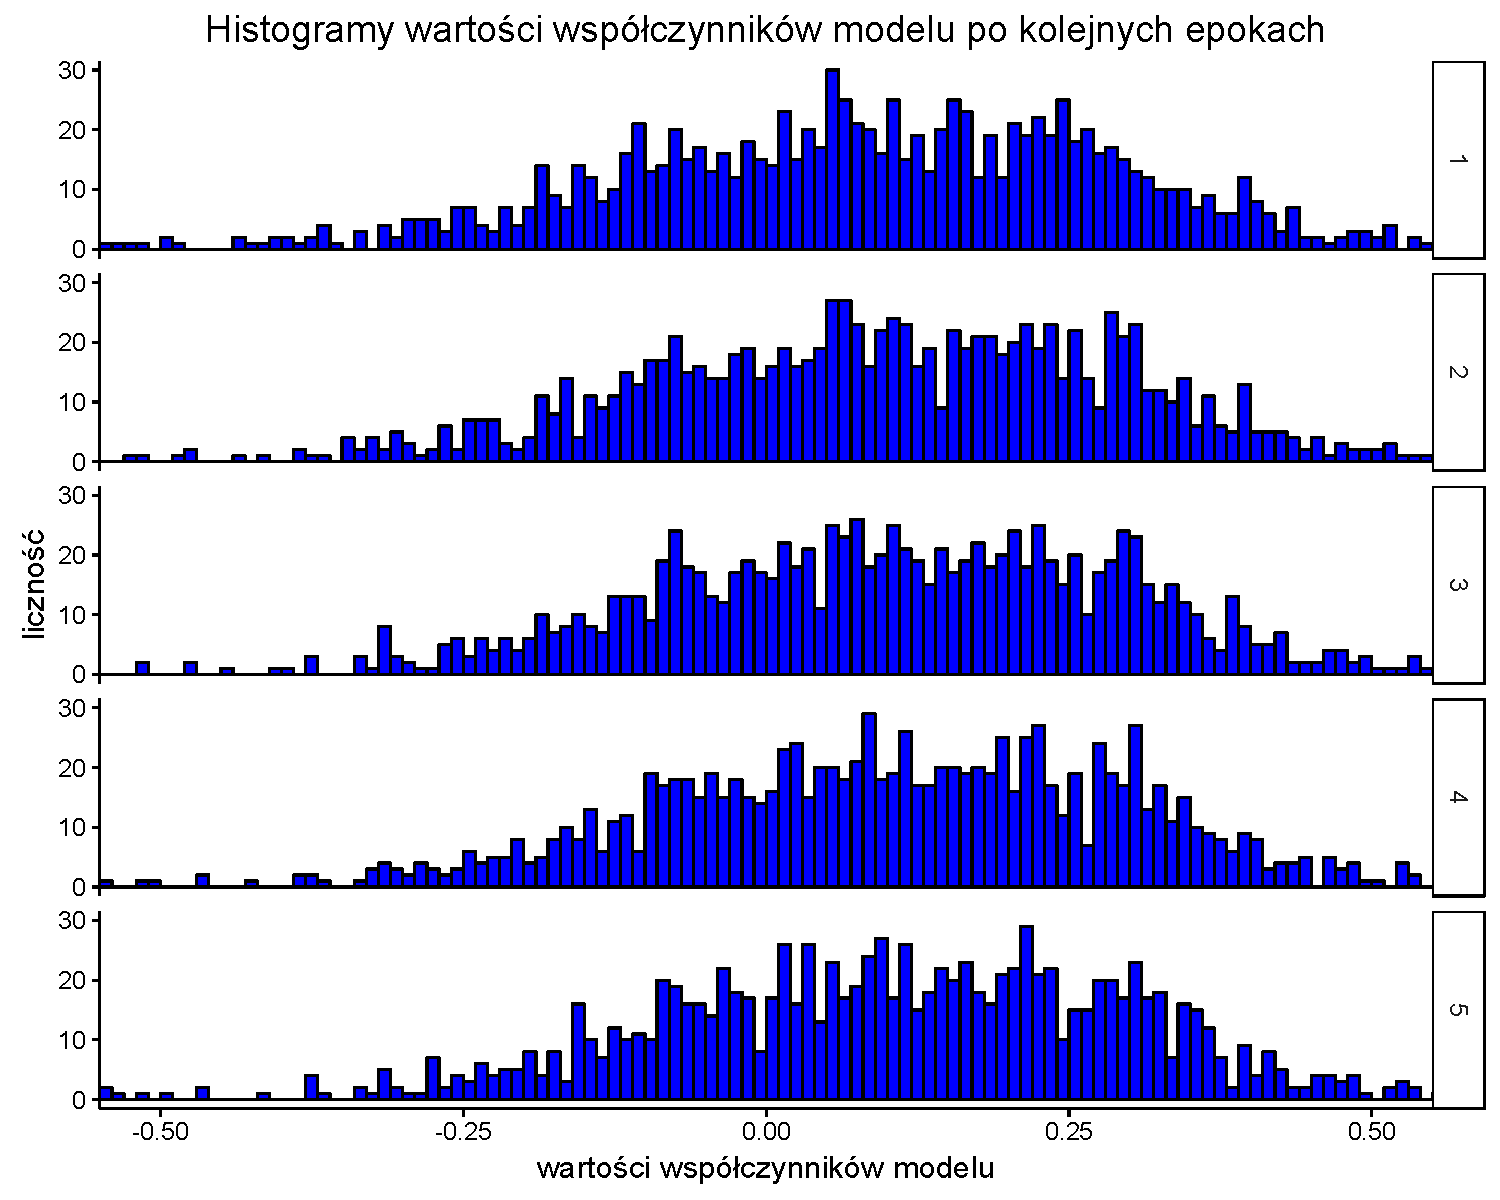
\includegraphics[width=0.95\textwidth, height = 280pt]{Obrazki/analiza/hist_overt_t.pdf}
\caption{\label{fig:hist1} Histogram wartości współczynników w modelu Coxa proporcjonalnych hazardów po kolejnych epokach. Współczynniki uzyskano dzięki wykorzystaniu algorytmu stochastycznego spadku gradientu, w którym ciąg odpowiadający za długość kroku to $\alpha_t = 1/t$.}
\ \\
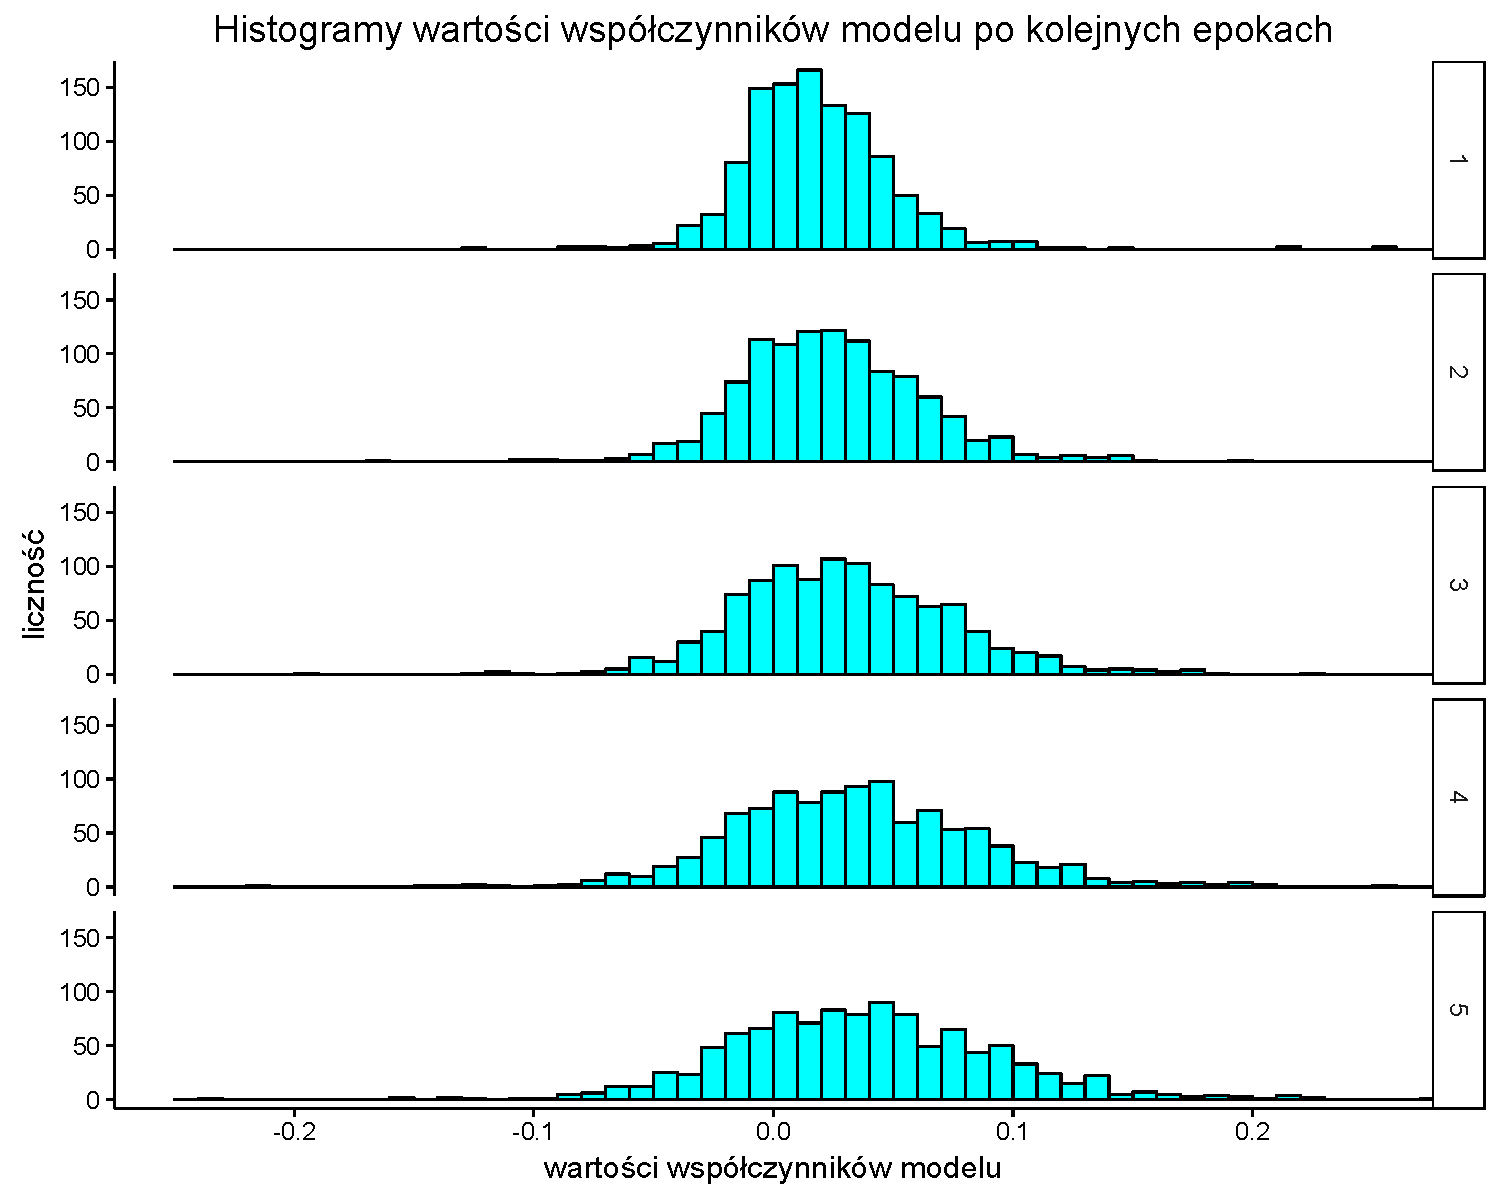
\includegraphics[width=0.95\textwidth, height = 280pt]{Obrazki/analiza/hist_over_50sqrt_t.pdf}
\caption{\label{fig:hist2} Histogram wartości współczynników w modelu Coxa proporcjonalnych hazardów po kolejnych epokach. Współczynniki uzyskano dzięki wykorzystaniu algorytmu stochastycznego spadku gradientu, w którym ciąg odpowiadający za długość kroku to $\alpha_t = 1/50\sqrt{t}$.}
\end{figure}
\begin{figure}[!ht]
\centering
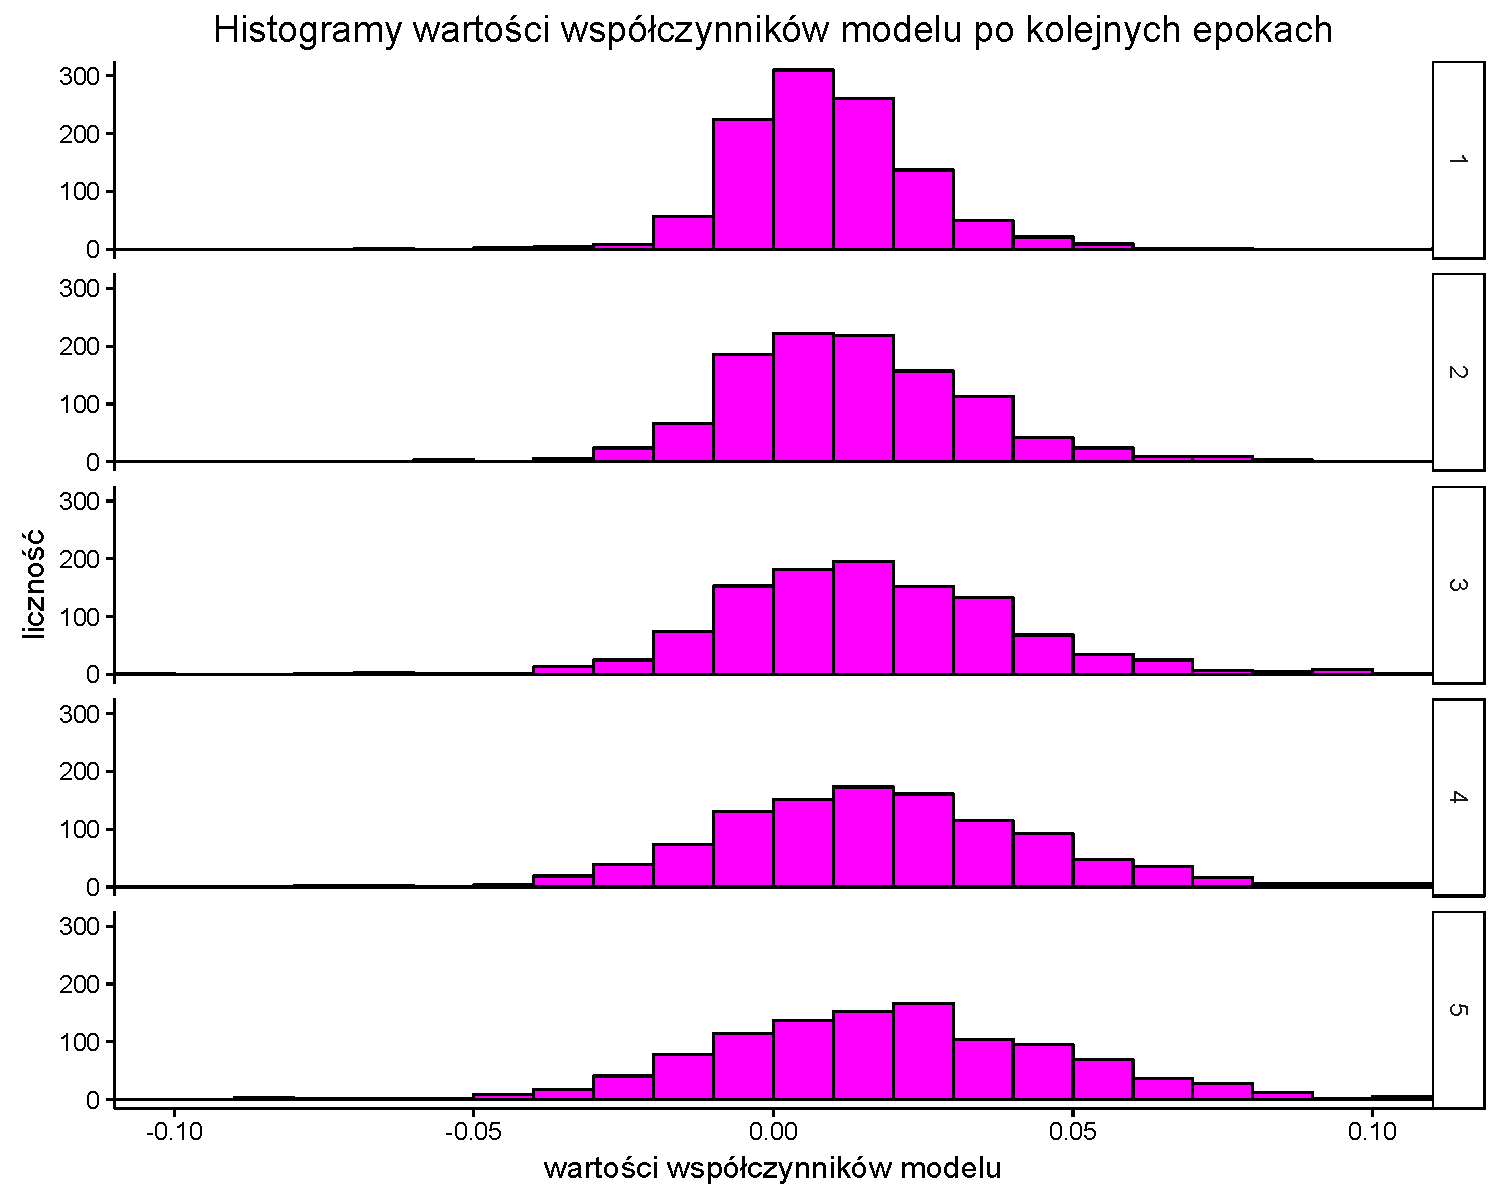
\includegraphics[width=0.95\textwidth, height = 280pt]{Obrazki/analiza/hist_overt_100sqrt_t.pdf}
\caption{\label{fig:hist3} Histogram wartości współczynników w modelu Coxa proporcjonalnych hazardów po kolejnych epokach. Współczynniki uzyskano dzięki wykorzystaniu algorytmu stochastycznego spadku gradientu, w którym ciąg odpowiadający za długość kroku to $\alpha_t = 1/100\sqrt{t}$.}
\ \\
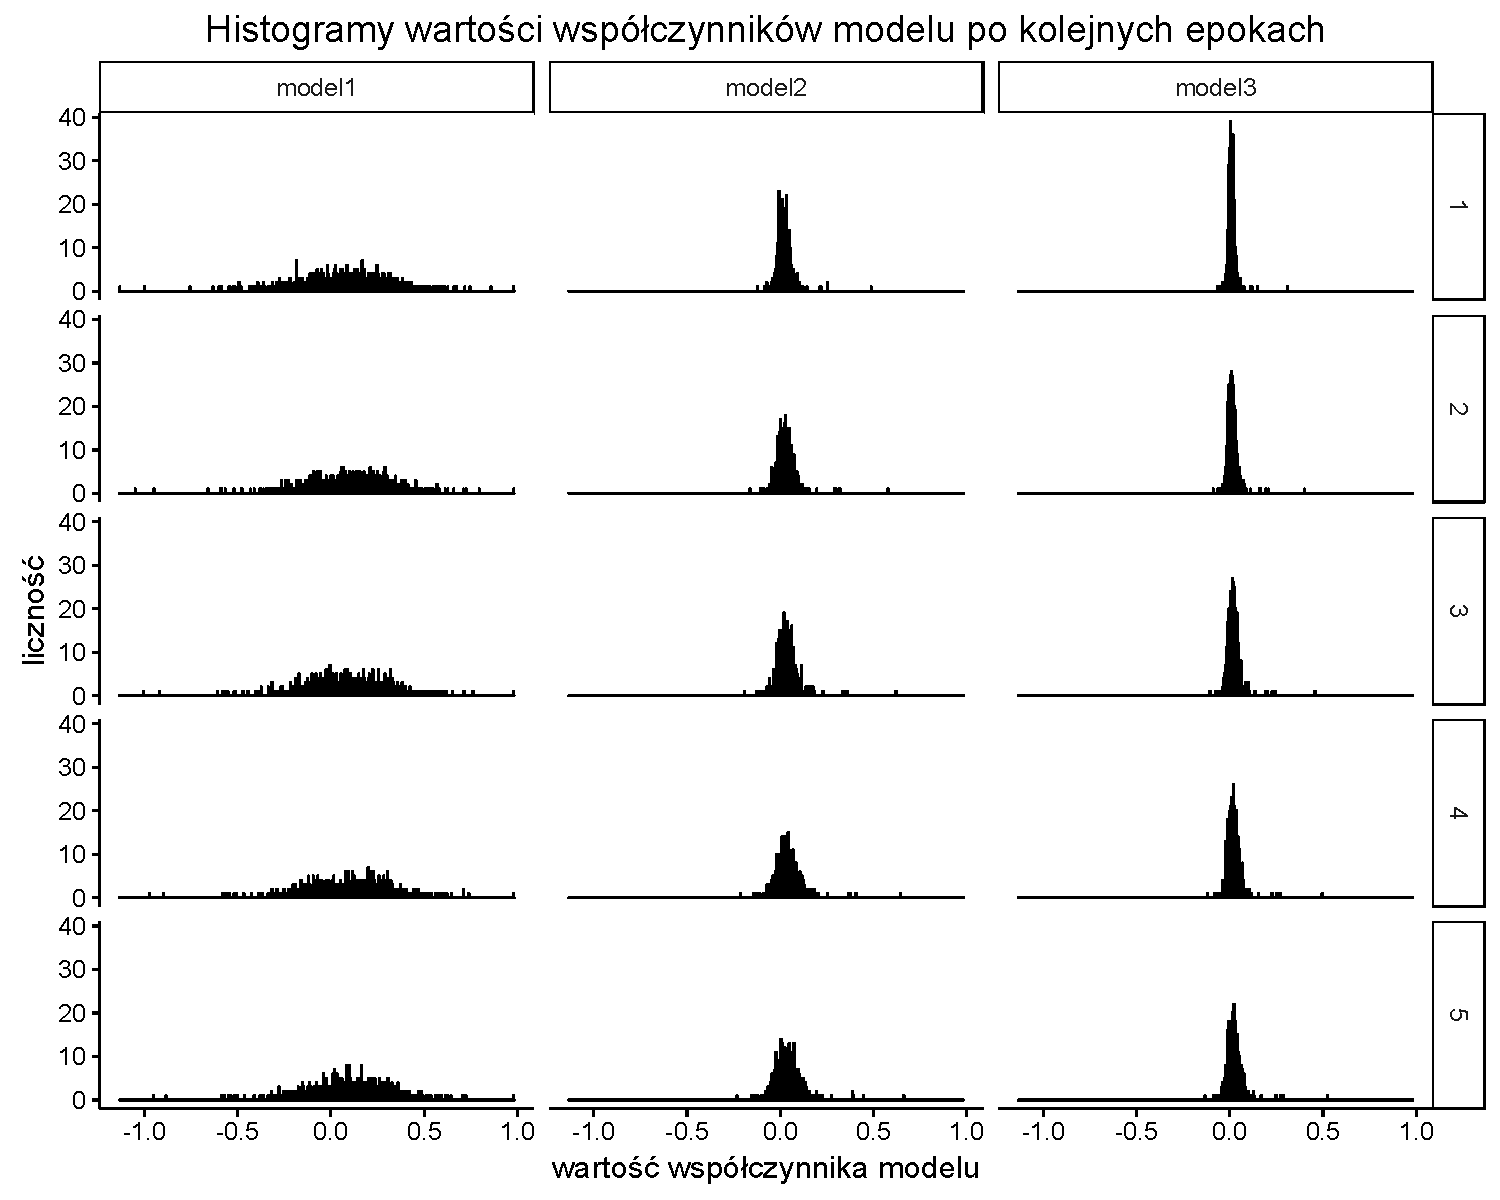
\includegraphics[width=0.95\textwidth, height = 260pt]{Obrazki/analiza/hist_together.pdf}
\caption{\label{fig:hist4} Porównanie histogramów wartości współczynników w modelu Coxa proporcjonalnych hazardów po kolejnych epokach. Współczynniki uzyskano dzięki wykorzystaniu algorytmu stochastycznego spadku gradientu, w którym kolejne ciągi odpowiadający za długość kroku to odpowiednio: $\alpha_{model1} = 1/t, \alpha_{model2} = 1/50\sqrt{t},  \alpha_{model3} = 1/100\sqrt{t}$.}
\end{figure}


\begin{figure}[!ht]
\centering
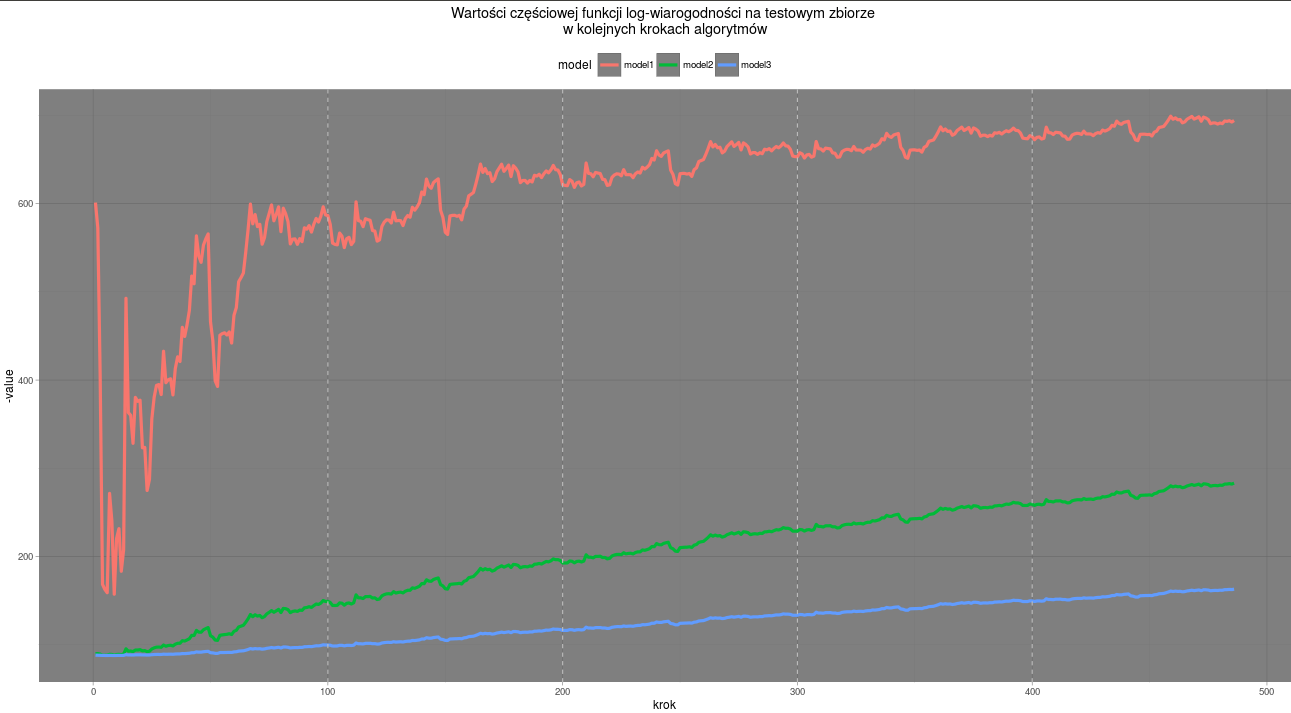
\includegraphics[width=0.95\textwidth, height = 280pt]{Obrazki/analiza/wartosci_loglik_test_ver_minus.png}
\caption{\label{wykres5}}
\ \\
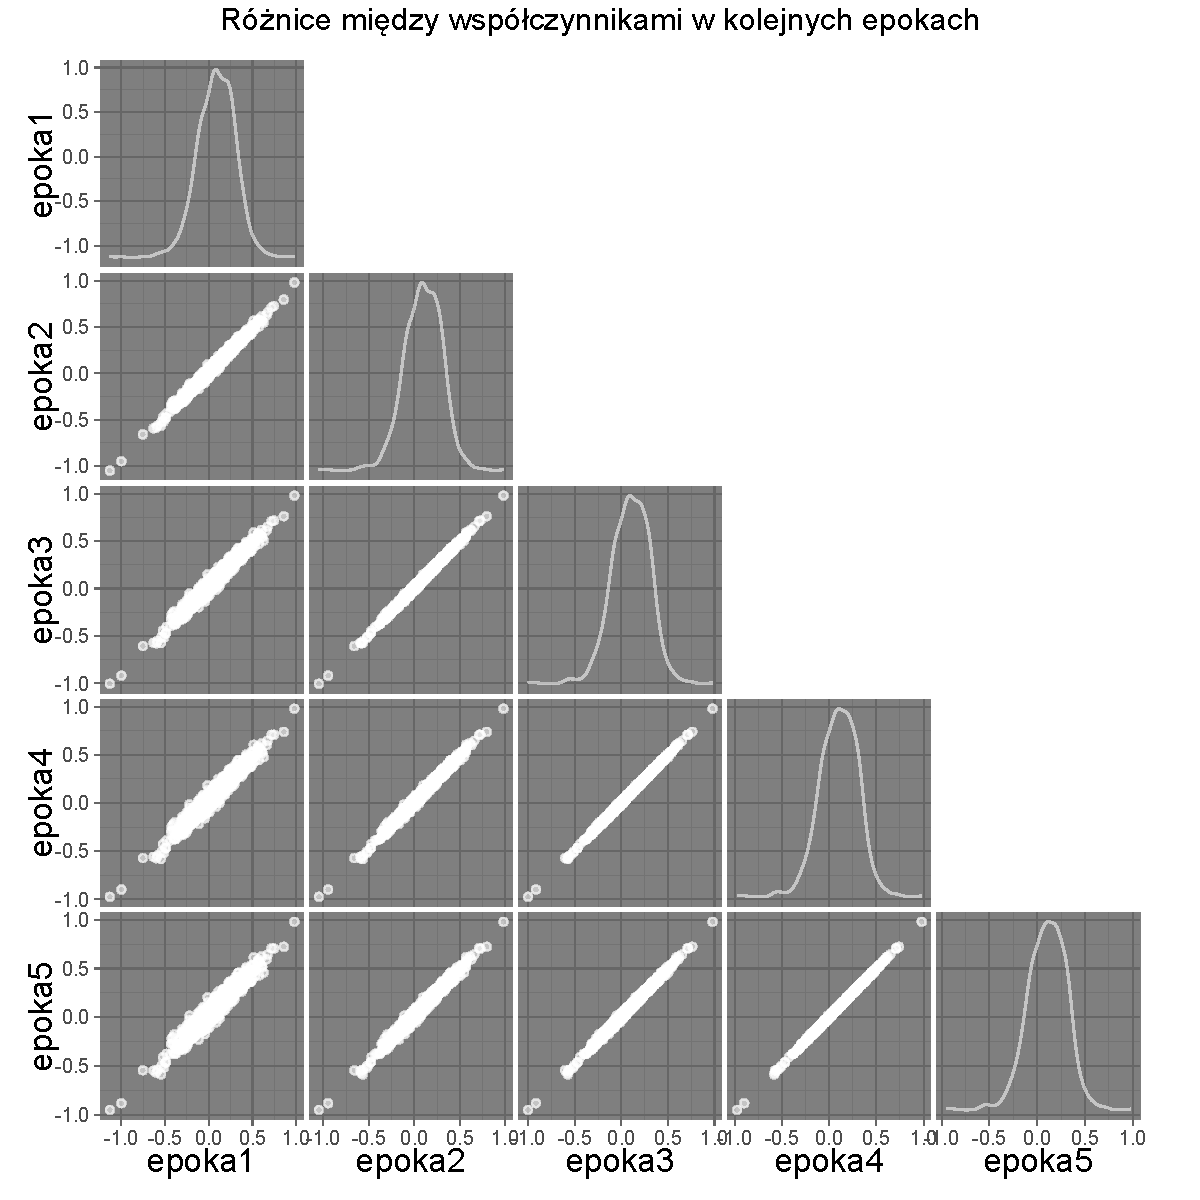
\includegraphics[width=0.95\textwidth, height = 280pt]{Obrazki/analiza/ggpairs_2.pdf}
\caption{\label{wykres6}}
\end{figure}

\subsubsection{Rezultaty analizy przeżycia}

Niemożliwe było sprawdzenie założeń modelu dotyczących proporcjonalności
hazardu, gdyż zakładano napływającą postać danych (stąd podział danych
na 100 grup). Dla takiej postaci pojawiania się danych ciężko także
mówić o jakiejkolwiek diagnostyce poprawności dopasowania modelu i
dokładności otrzymanych współczynników. Nie stworzono teorii
pozwalającej badać istotność statystyczną otrzymanych współczynników w
modelu, jednak założono, że współczynniki dostatecznie odległe od \(0\)
można uznać za istotnie wpływające na czas życia pacjenta. Współczynniki
dodatnie oznaczają zwiększenie hazardu pacjenta posiadającego mutację w
danym genie w stosunku do pacjentów nie posiadających mutacji w danym
genie. Współczynniki ujemne oznaczają zmniejszenie hazardu pacjenta
posiadającego mutację w danym genie w stosunku do pacjentów nie
posiadających mutacji w danym genie. Wzrost proporcji hazardu można
otrzymać dla danego genu poprzez obłożenie współczynnika funkcją
wykładniczą o wykładniku \(e\).


Wyniki estymacji dla genów zawierających największe co do modułu
współczynniki (pochodzące z modelu dającego największą wartość częściowej funkcji log-wiarogodności konstruowanej na bazie dwóch ostatnich zaobserwowanych podzbiorów danych) można znaleźć w Tabeli \ref{tabelka}.

\begin{table}[ht]
\centering
\begin{tabular}{rrr}
  \toprule
 & $\beta$ & $e^{\beta}$ \\ 
  \toprule
EGFR & 0.97 & 2.63 \\ 
  ATP2B2 & 0.86 & 2.35 \\ 
  NDST4 & 0.73 & 2.08 \\ 
  TP53 & 0.71 & 2.04 \\ 
  CHRM2 & 0.67 & 1.95 \\ 
  C3 & 0.66 & 1.93 \\ 
  LAMC3 & 0.61 & 1.85 \\ 
  PCDH9 & 0.61 & 1.84 \\ 
  LRRC4C & 0.61 & 1.84 \\ 
  C15orf2 & 0.60 & 1.83 \\ 
  ATG2A & 0.58 & 1.78 \\ 
  GLI2 & 0.58 & 1.78 \\ 
  KEAP1 & 0.57 & 1.76 \\ 
  Unknown & 0.56 & 1.75 \\ 
  KIAA1409 & 0.56 & 1.75 \\ 
  LTBP2 & 0.55 & 1.73 \\ 
  GRIA4 & 0.53 & 1.70 \\ 
  ADAMTSL1 & 0.53 & 1.70 \\ 
  NTRK3 & 0.52 & 1.69 \\ 
  ZFAT & 0.52 & 1.68 \\ 
  CDKN2A & 0.51 & 1.67 \\ 
  TMEM132D & 0.51 & 1.67 \\ 
  CDH9 & 0.50 & 1.65 \\ 
  FAM5C & 0.50 & 1.65 \\ 
  KCNA4 & 0.50 & 1.65 \\ 
  MUC16 & 0.50 & 1.64 \\ 
  GPR133 & 0.50 & 1.64 \\ 
  ZNF804B & 0.49 & 1.64 \\ 
  LRRIQ1 & 0.49 & 1.63 \\ 
  ZMYM3 & -0.49 & 0.61 \\ 
  CTCF & -0.52 & 0.60 \\ 
  OTOF & -0.52 & 0.59 \\ 
  IDH1 & -0.53 & 0.59 \\ 
  CDH1 & -0.55 & 0.58 \\ 
  DNAH17 & -0.59 & 0.56 \\ 
  PLXNC1 & -0.60 & 0.55 \\ 
  DLGAP2 & -0.61 & 0.54 \\ 
  BCORL1 & -0.75 & 0.47 \\ 
  FLRT2 & -1.00 & 0.37 \\ 
  BRAF & -1.14 & 0.32 \\ 
   \bottomrule
\end{tabular}
\caption{\label{tabelka}Współczynniki oraz stosunki hazardów ($e^{\beta}$) w modelu proporcjonalnych hazardów Coxa dla modelu dającego największą wartość funkcji częściowej log-wiarogodności na zbiorze testowym. }
\end{table}
